In questo documento si espone il progetto sviluppato dal sottoscritto per il corso di Intelligenza Artificiale presso l'Università degli Studi di Bergamo.
Il progetto consiste nel confrontare diverse tecniche di classificazione binaria di immagini provenienti da diverse TAC al cervello per il riconoscimento di un tumore.\\
Si ha a disposizione un dataset in formato csv che racchiude le caratteristiche dimensionali e statistiche delle immagini raccolte dalle TAC.\\

\begin{figure}[!htb]
	\minipage{0.24\textwidth}
	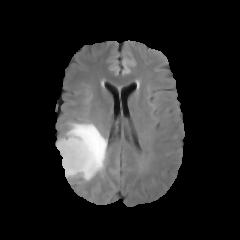
\includegraphics[width=\linewidth]{image/Image1.jpg}
	\label{fig:immagine01}
	\endminipage\hfill
	\minipage{0.24\textwidth}
	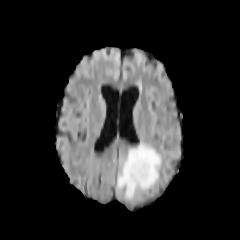
\includegraphics[width=\linewidth]{image/Image2.jpg}
	\label{fig:immagine2}
	\endminipage\hfill
	\minipage{0.24\textwidth}
	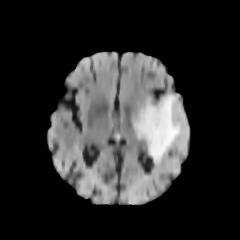
\includegraphics[width=\linewidth]{image/Image3.jpg}
	\label{fig:immagine3}
	\endminipage\hfill
	\minipage{0.24\textwidth}%
	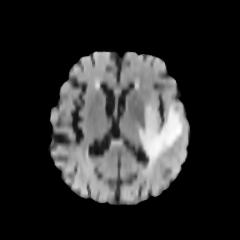
\includegraphics[width=\linewidth]{image/Image4.jpg}
	\label{fig:immagine04}
	\endminipage
	\caption{Esempio di quattro TAC al cervello}
\end{figure}

Il file \textit{bt\_dataset\_t3.csv}, disponibile sul sito \textit{www.kaggle.com}, contiene le seguenti colonne (feature):
\begin{itemize}
	\item Nome dell'immagine (ImageX, dove X indica il numero della TAC)
	\item Valori di target (1 se è un tumore, 0 se non è un tumore)
	\item Media
	\item Varianza
	\item Deviazione Standard
	\item Skewness
	\item Curtosi
	\item Contrasto (intensità)
	\item Energia
	\item ASM (Angular Second Moment), ovvero un indice che rappresenta l'uniformità del livello di grigio nell'immagine
	\item Entropia
	\item Omogeneità
	\item Dissimilarità
	\item Correlazione
	\item Ruvidezza dell'immagine
\end{itemize}
In pratica le macchie presenti nelle TAC al cervello vengono studiate come distribuzioni statistiche estrapolate da analisi di immagini.\\
L'obiettivo è quindi utilizzare le tecniche KNN, Regressione Logistica, Kernel SVM e Multi-Layer Perceptron per riconoscere quali macchie possono essere considerate tumori e quali no.\\
Gli strumenti utilizzati sono diversi moduli Python, come \textit{Pandas}, \textit{Scikit-Learn} e \textit{Matplotlib}.\\
Le diverse tecniche son state implementate in quattro file di estensione .py per facilità di lettura. In questo documento si illustreranno i punti chiave dei codici.\\
Prima di procedere con l'implementazione delle tecniche di classificazione qui sopra indicate, è stato necessario fare \textit{preprocessing} sul dataset in quanto vi sono colonne non utili (come il nome delle immagini) e alcuni dati NaN e infiniti che non sono compatibili con gli algoritmi.